\setcounter{chapter}{5} %this gives Chapter 6
\chapter{Experiments with the Sandia trap}
\label{chapter:sandia}

This chapter and the next summarise the results of experiments with trapped \Ca{40} ions in the Sandia trap. The current chapter first describes the photoionisation and trapping. This is followed by accounts of the experiments to measure the trap lifetime and the vibrational frequencies, and trapping of multiple ions. Measurement of the heating rate in the trap and shuttling single ions along the trap axis are presented in Chapter~\ref{chapter:heating}.

\section{Ion loading}
\label{sec:ionload}
In our ion loading scheme, 4 different laser frequencies are used: a 423\nm\,beam excites the neutral \CaI{} atoms. A 389\nm\,beam provides further excitation for photoionisation. A pair of beams (397\nm\, and 866\nm) are used for Doppler-cooling and detection of the ion (see the relevant energy level structure of \CaI{} and \Ca{} in Figure~\ref{fig:levels}).

One difficulty was that before any ions had actually been captured, it was hard to check whether certain parts of the experimental equipment were functioning correctly. The applied DC and RF voltages can be measured only outside the vacuum chamber, so there is no direct method to check the true values of voltages on the electrodes. The laser beams need to be precisely guided through the trapping position of the electromagnetic field, but with no signal the correct position can only be estimated.


It was only with difficulty that the correct working procedure for the Sandia trap was discovered. There was initially a period of 2 months during which all attempts to load ions and detect fluorescence failed. During this period various aspects of the apparatus were honed and improved, but ultimately the failure to trap ions was caused
mainly by one oversight. When looking for the possibly weak fluorescence signals associated with the first loading of ions, we adopted the standard practice of using a differential detection scheme, somewhat like `phase-sensitive detection'. The 866\nm\, laser was pulsed on and off for periods of 50 ms, and the photomultiplier count signal for each ``off'' period was substracted from the signal for the neighbouring ``on'' period. This suppresses noise associated with background scatter and laser intensity fluctuations. However, the combination of collisional heating (from the background gas and the neutral atom beam) and intrinsic electric field noise in the trap meant that trapped ions could not survive in the trap with the Doppler cooling thus switched off for periods of 50 ms. This was exacerbated by a poor choice of DC electrode voltages, before the backplane electrode was accounted for in the numerical model (this poor choice did not make the trap completely unstable, but it reduced the trap depth). Once we optimised the voltages, reduced the atomic beam flux and, most importantly, went over to continuous Doppler cooling, ions were loaded satisfactorily. Then was it possible to adjust the DC voltages for good compensation and thus achieve the
most stable trap.

The University of Michigan group experienced severe problems with a trap of the same design and, to our knowledge, either never or only briefly managed to trap ions in it. The NIST group loaded ions in a similar trap but found the trapped ions did not stay in one place, suggesting that the electric field environment was quite unstable owing to surface and materials issues. The University of Innsbruck, Austria group was unable to load ions in a trap of the same design. Their system was different from ours as the trap is mounted much closer to the observation window (dielectric surface) and the pressure in their container was some orders of magnitude higher.


%%%%%%%%%
%After some 2 months of exploring different experimental control parameters (laser beam positions, laser detunings, electrode voltages, different Doppler cooling pulse sequences), we successfully loaded \Ca{} ions into the Sandia trap. The significant factors in our trap turned out to be the use of continuous Doppler-cooling, and using large detuning from the resonance. Both issues are connected to the very high motional  energy of the ions (large amount of micro-motion) after loading, because of the lack of stray electric field compensation.
%
% Continuous Doppler-cooling was needed to provide enough cooling to counteract the the heating experienced by the ion. Initially, pulsed Doppler cooling was used, in a pattern of 50\ms\,Doppler-cooling followed by 50\ms\,background scatter measurement, during which the 866\nm\,beam was turned off. In this situation no trapped ion signal was observed, probably because the ions escaped from the trap after a very short time due to the rapid heating.

%During ion loading large detuning from the atomic resonance was needed since the effective linewidth is much greater than the natural width. Ions loaded before correct field compensation generally had fluorescence spectra with Doppler broadening of several hundred \MHz.

Figure~\ref{fig:signal854}(a) shows a recorded fluorescence signal as a function of time, during the ion loading. The photoionisation and Doppler-cooling lasers were on. Due to the filters placed in front of the PMT, the recorded signal corresponds only to the observed 397\nm\,light. All other wavelengths were filtered out. The signal shows very short time intervals when the ion is fluorescing, before it drops to the background level. Initially we interpreted this as the ion escaping from the trap because of collisions with other neutral \CaI{} atoms, or other \Ca{} ions in the trapping region. Collisions with \CaI{} atoms were ruled out because the fluorescence signal became continuous (not dropping back to the background level), when the \CaI{} oven was left on and the photoionisation lasers were blocked after trapping. 
%Collisions with ions were also ruled out, because the fluorescence signal did not change when the photoionisation beams were left on, but the \CaI{} oven was turned off (and thus the source of neutral \CaI{} in the trapping region was cut off) after trapping.

The correct mechanism for the observed fluorescence pattern was eventually  recognised to be off-resonant excitation of the \soh-\pth\, transition by the 389\nm\, photoionisation beam, which transfers the population to the metastable \dfh\, state, thus shelving the ion. To eliminate this effect, an 854\nm\, ``deshelving'' laser was used. This transfers the ion from the \dfh\, to the \pth\, state, to eventually decay back to the ground state, and enable the Doppler cooling lasers to interact with the ion. The effect of this additional beam is shown in Figure~\ref{fig:signal854}(b). The \CaI{} oven, the photoionisation and Doppler cooling lasers were used in the same manner as in Figure~\ref{fig:signal854}(a). With the ``deshelving'' beam the observed ion lifetimes were comparable to the lifetimes when the photoionisation beams are turned off after ion capture.

This shelving effect of the 389\nm\, beam is not an issue when loading only a single ion, since one can always block the photoionisation beams. It is very important, however, when loading multiple ions, as described in Section \ref{sec:multiions}.


%\begin{figure}[!t]
%\centering
%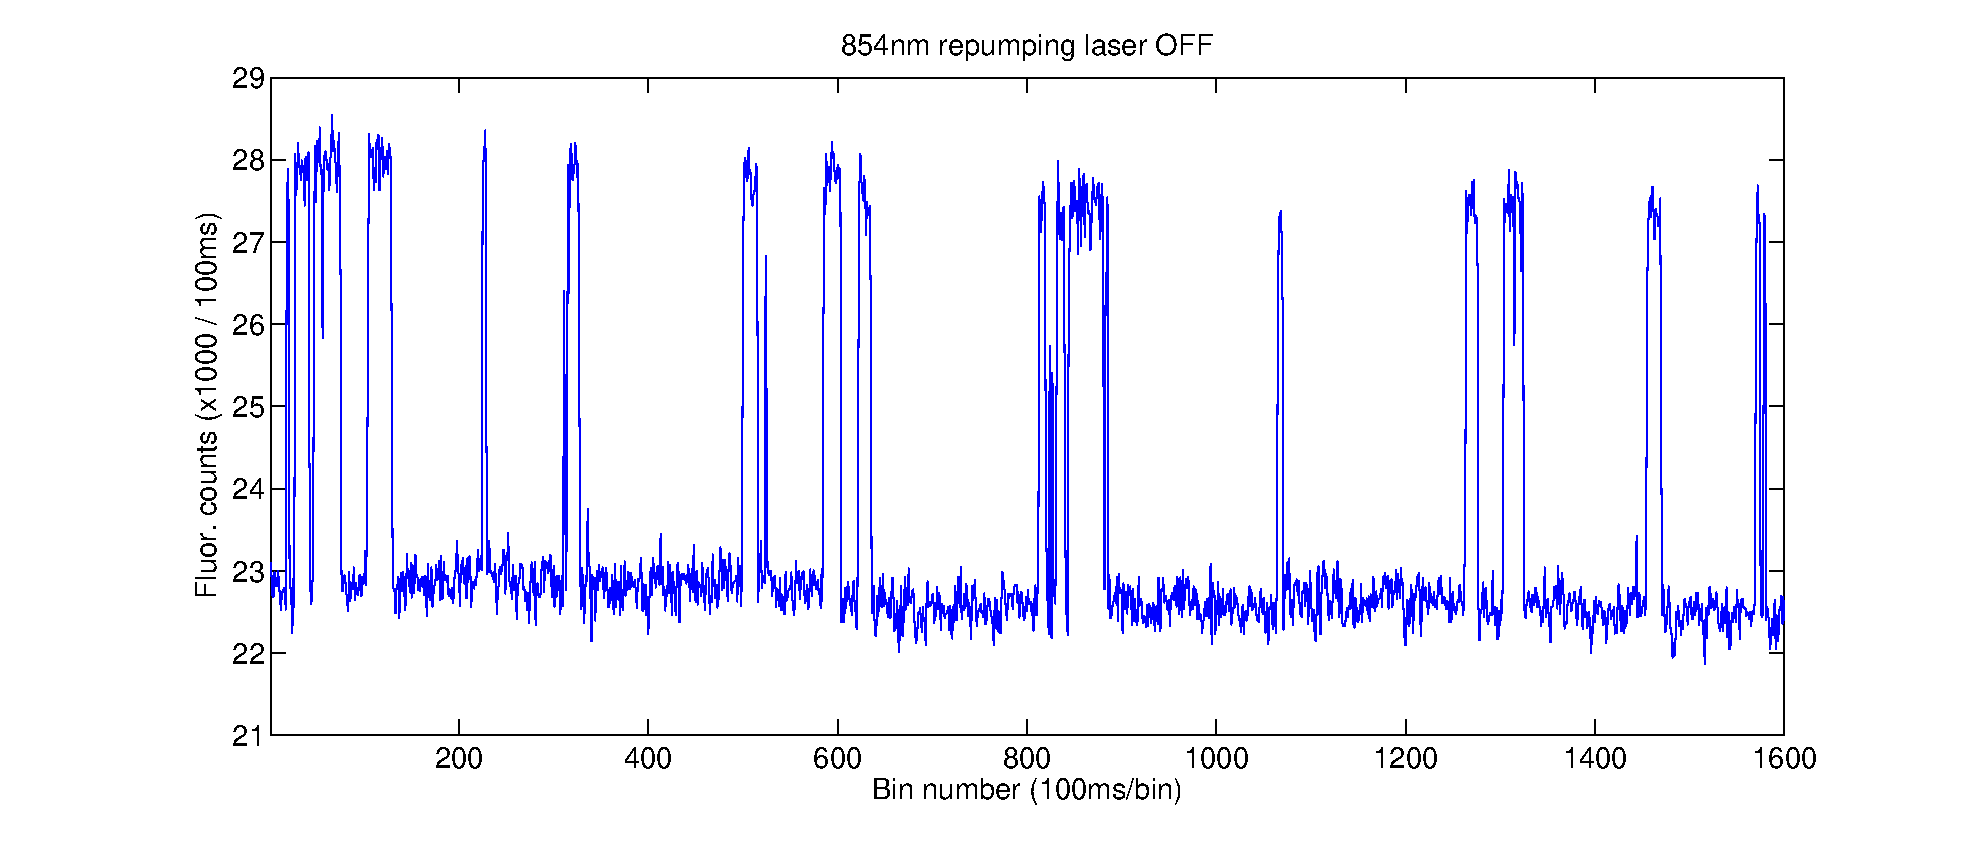
\includegraphics[width=14.5cm]{chapter6/854effect/854effect_a}
%\caption[Trapped ion fluorescence during loading, without 854\nm\, laser beam]{Trapped ion fluorescence signal. The photon counts are plotted as a function of recorded bin number (100\ms\, per bin). There are a large number of quantum jumps present, most of which are attributed to far off-resonant shelving by the 389\nm\, photoionisation beam (see text). The 854\nm\, beam is off, while the 389\nm, 423\nm, 397\nm, 866\nm\, beams are on continuously.}
%\label{fig:signal854off}
%\end{figure} 
%
%\begin{figure}[!h]
%\centering
%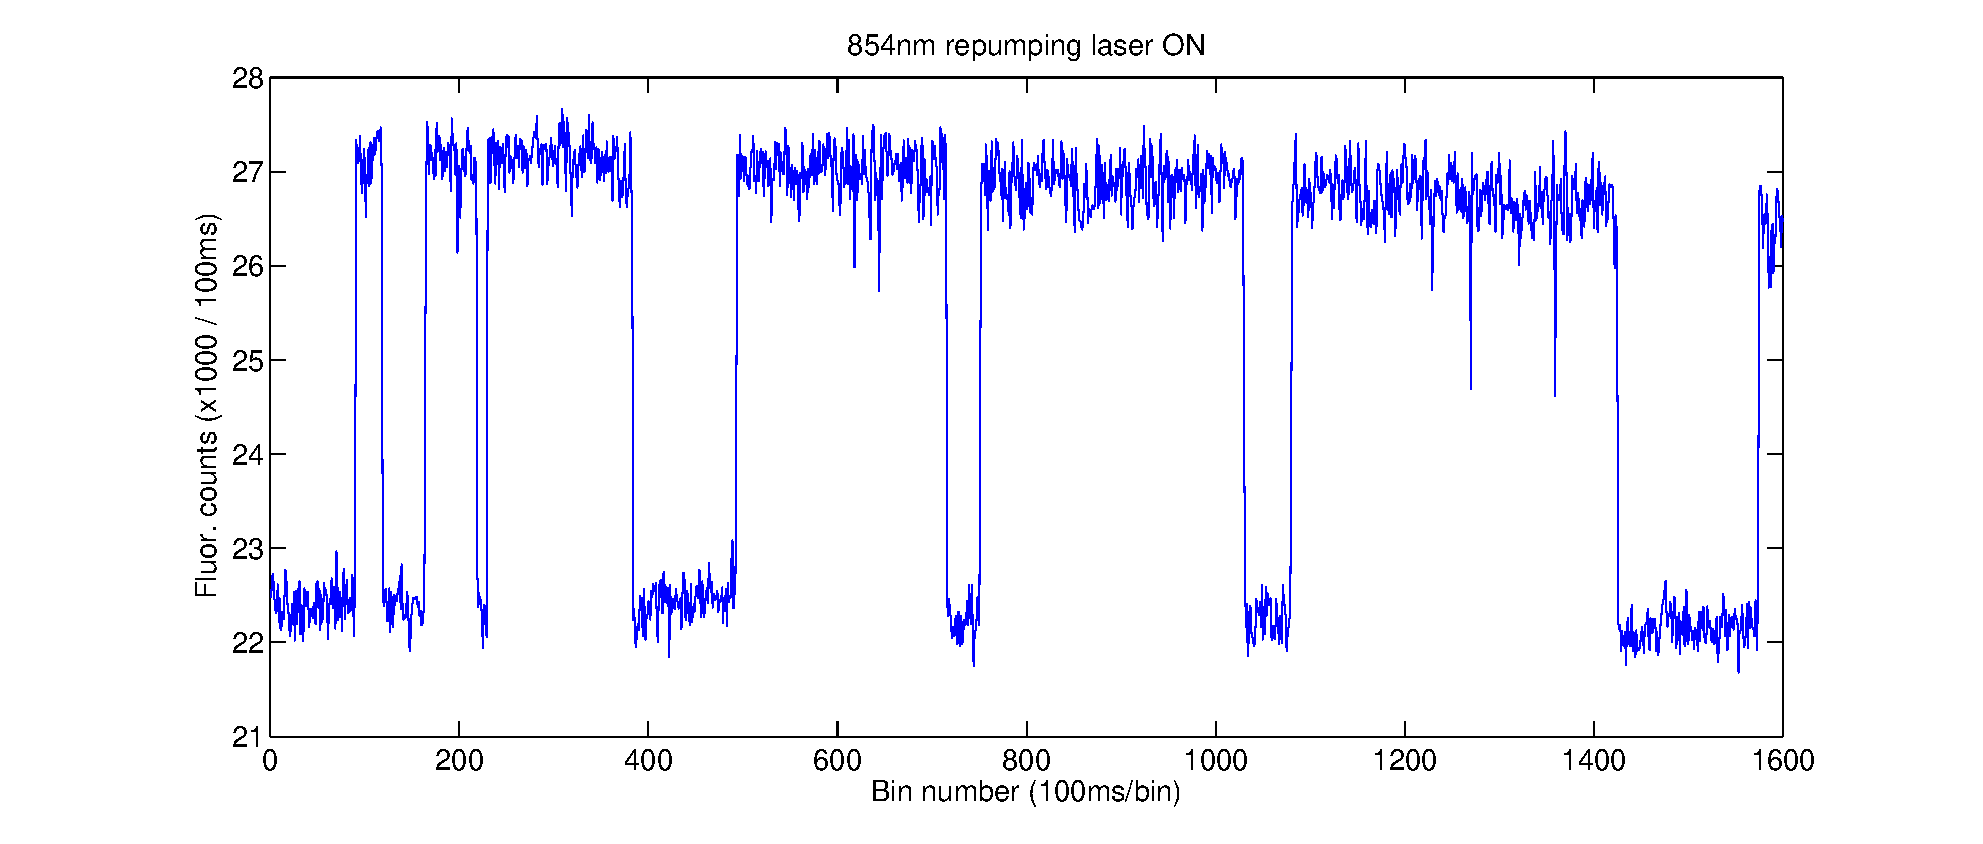
\includegraphics[width=14.5cm]{chapter6/854effect/854effect_b}
%\caption[Trapped ion fluorescence during loading, with 854\nm\, laser beam]{Trapped ion fluorescence signal during loading, when an 854\nm\, laser beam is applied in addition to those present for the fluorescence shown in Figure~\ref{fig:signal854off}. The photon counts are plotted as a function of recorded bin number (100\ms\, per bin). The number of quantum jumps is reduced compared to Figure \ref{fig:signal854off}, which was recorded in the same experimental run. The remaining jumps are due to  newly captured and lost ions.}
%\label{fig:signal854on}
%\end{figure} 

\begin{figure}[!t]
\begin{center}
$\begin{array}{rl}
\mbox{\bf (a)} & 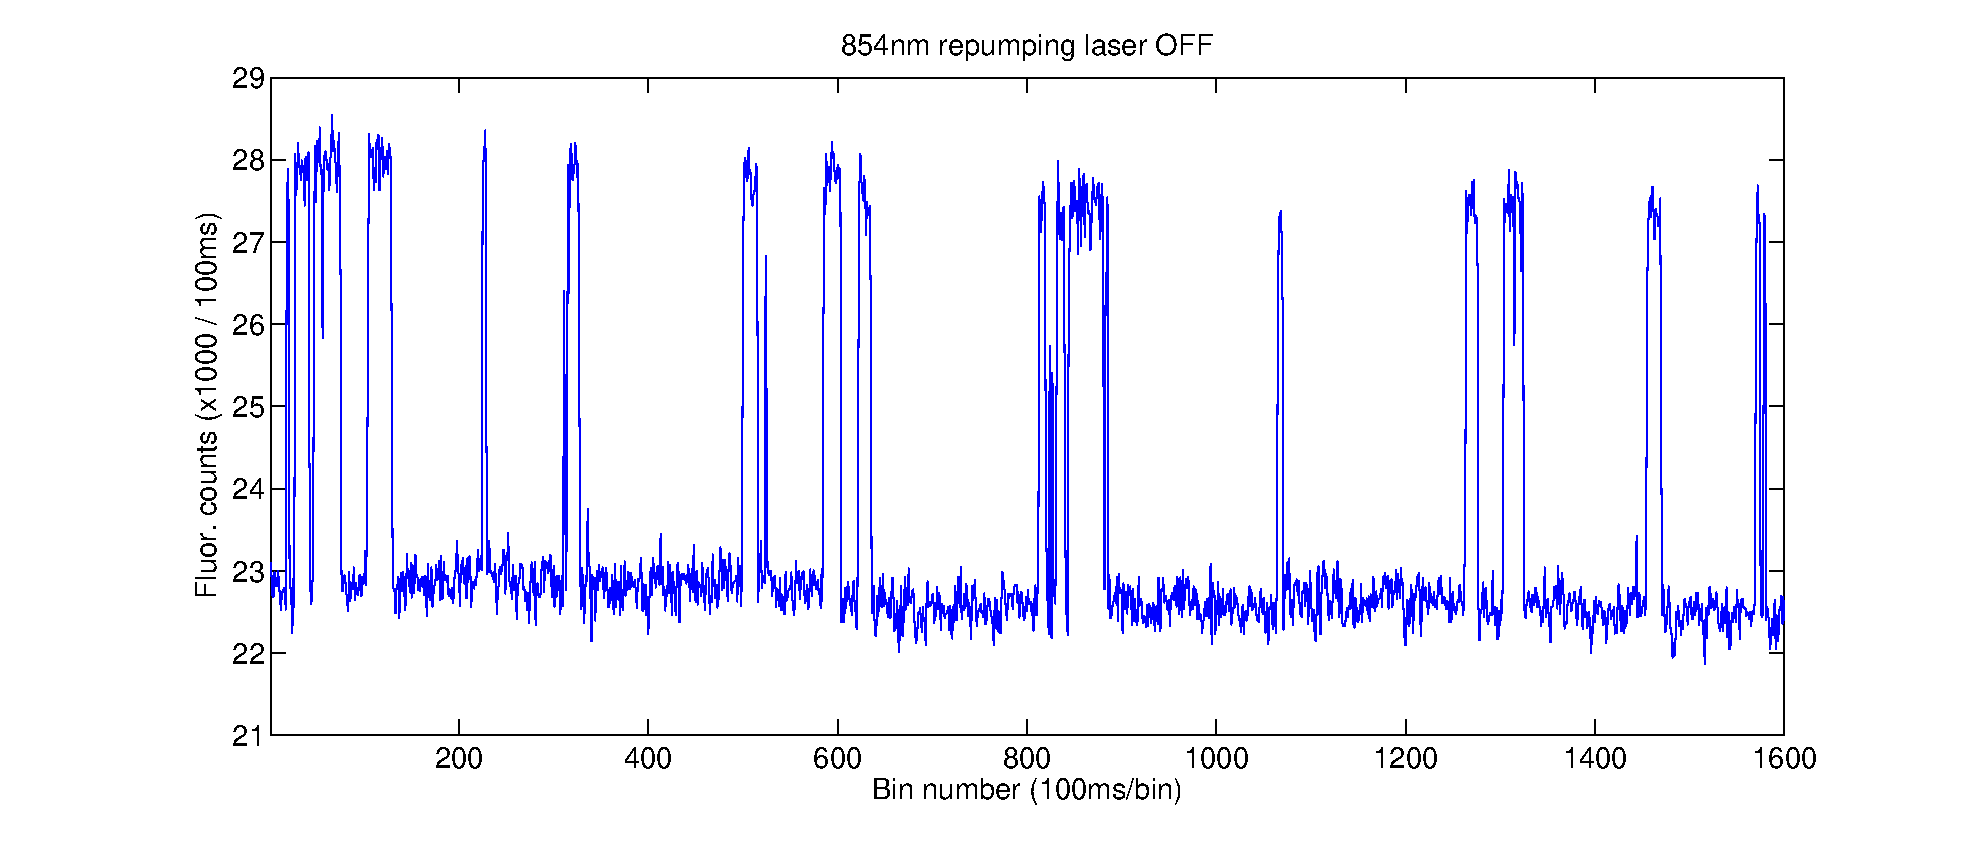
\includegraphics[width=14.5cm]{chapter6/854effect/854effect_a}\\
\mbox{\bf (b)} & 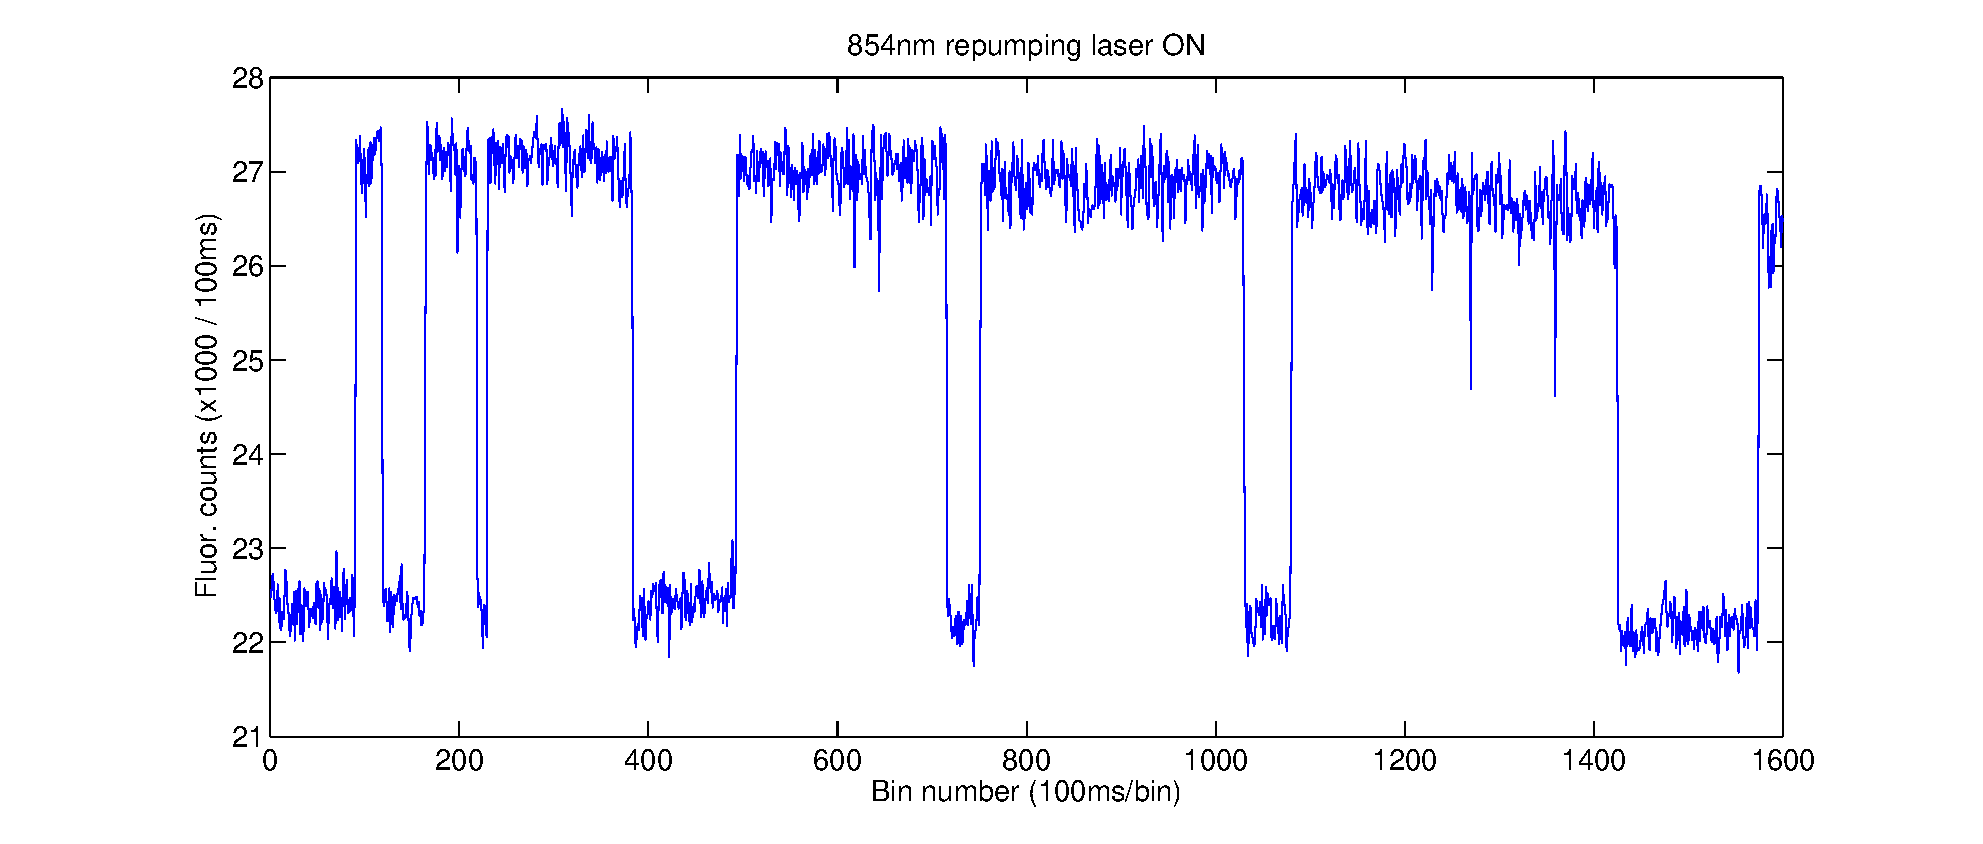
\includegraphics[width=14.5cm]{chapter6/854effect/854effect_b} \\
\end{array}$
\end{center}
\caption[Trapped ion fluorescence during loading, effect of 854\nm\, laser]{Trapped ion fluorescence signal during loading (a) without 854\nm\, beam b) with the 854\nm\, beam on.  The recorded photon count is plotted as a function of recorded bin number (100\ms\, per bin). All photoionisation and Doppler-cooling lasers (389\nm, 423\nm, 397\nm, 866\nm) are on continuously on both plots. On (a) there are a large number of quantum jumps present, most of which are attributed to far off-resonant shelving by the 389\nm\, photoionisation beam (see text). On (b) the number of quantum jumps is reduced due to the deshelving effect of the 854\nm\, laser beam. The remaining jumps in fluorescence are likely to signal newly captured and then lost ions.}
\label{fig:signal854}
\end{figure} 



\section{Micro-motion compensation}
\label{sec:micromotioncomp}

Once ion loading is reliable, one can attempt to compensate stray electric fields. Compensation is achieved by adjusting the DC electrode voltages, in order to make the DC potential minimum coincide with the RF potential minimum. 

The compensation is usually done in two steps. Initially the fields are very badly compensated and the ion has a large amount of micro-motion. First a rough compensation is attempted and then it is fine-tuned by a correlation method.

In the case of a large amount of micro-motion, the fluorescence spectrum is observed while scanning the 397\nm\, laser frequency on the red side of the atomic resonance. The electrode voltages are adjusted so as to reduce the observed  Doppler broadening \cite{Stevens1999}. Figure~\ref{fig:397compensationscans} shows a pair of scans as an example for a Doppler-broadened and a relatively well compensated spectrum. 

\begin{figure}[!ht]
\centering
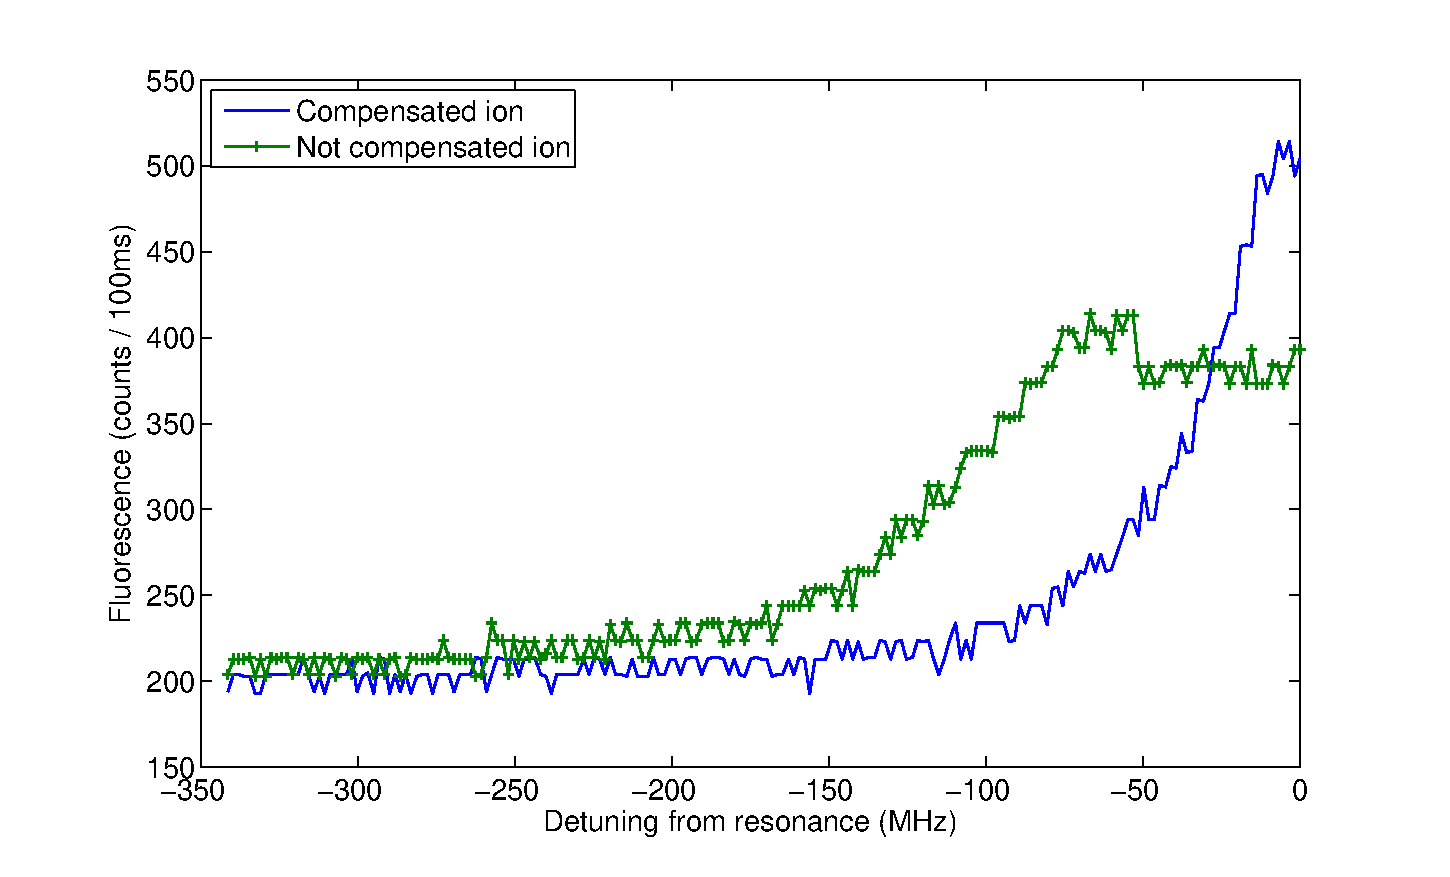
\includegraphics[width=14.5cm]{chapter6/rfcorr/compensation397_2}
\caption[Fluorescence spectra before and after stray field compensation]{A pair of experimental fluorescence spectra showing the Doppler-broadened profile before field compensation and the narrower profile after the crude field compensation described in the text. The photon counts are shown as a function of laser detuning. The detuning is calculated from the calibration shown in Table~\ref{tab:lasercalib}. \cversion }
\label{fig:397compensationscans}
\end{figure} 

When trapping the ion in the geometric centre of the trap, most of the time the middle DC electrode pair and the pairs next to them were used (electrode pairs \#3, \#4 and \#5, see Figure~\ref{fig:sandiatrap}). The horizontal 397\nm\, Doppler-cooling beam provides information about the micro-motion along the trap axis and out of the plane of the DC electrodes (Z and Y directions, respectively). The compensation in the Z and Y directions is done by adjusting the DC voltage on the \#3 and \#5 DC electrode pairs relative to the \#4 pair. This method will mainly adjust the Y compensation because of symmetry. However, the position of the RF pseudo-potential minimum needs to be matched mostly in the Y direction, because the RF field is much stronger in the Y than in the Z direction. Thus, generally good compensation is achieved by this symmetric adjustment of voltages.

Once the micro-motion is reduced, fine adjustment is achieved by RF-photon correlation \cite{Stacey2003}. The method is detailed in A. Myerson's first year report \cite{Myerson2007}, and a brief outline is given here.

The 397\nm\, laser is tuned to the half-fluorescence point on the red side of the atomic transition. The number of fluorescence photons detected is recorded as a function of their arrival time with respect to the RF cycle. In the case of good micro-motion compensation, the photon arrival times are independent of the RF cycle. However, in the case of micro-motion, the photon arrivals have a timing profile following the RF potential's sinusoidal change. Figure \ref{rfcorrelation} shows three example plots of under/over-compensated and well compensated photon arrival times. There are two cut-off thresholds on the time axis. The upper threshold is $\tau = 36.7\ns$, which corresponds to one cycle of the RF voltage at $\Omega_{RF} = 2\pi \times 27.25\MHz$. The origin of the lower threshold ($\tau =3.5\ns$) is not certain, but is possibly due to the reaction time of the electronics.

\begin{figure}[t]
\centering
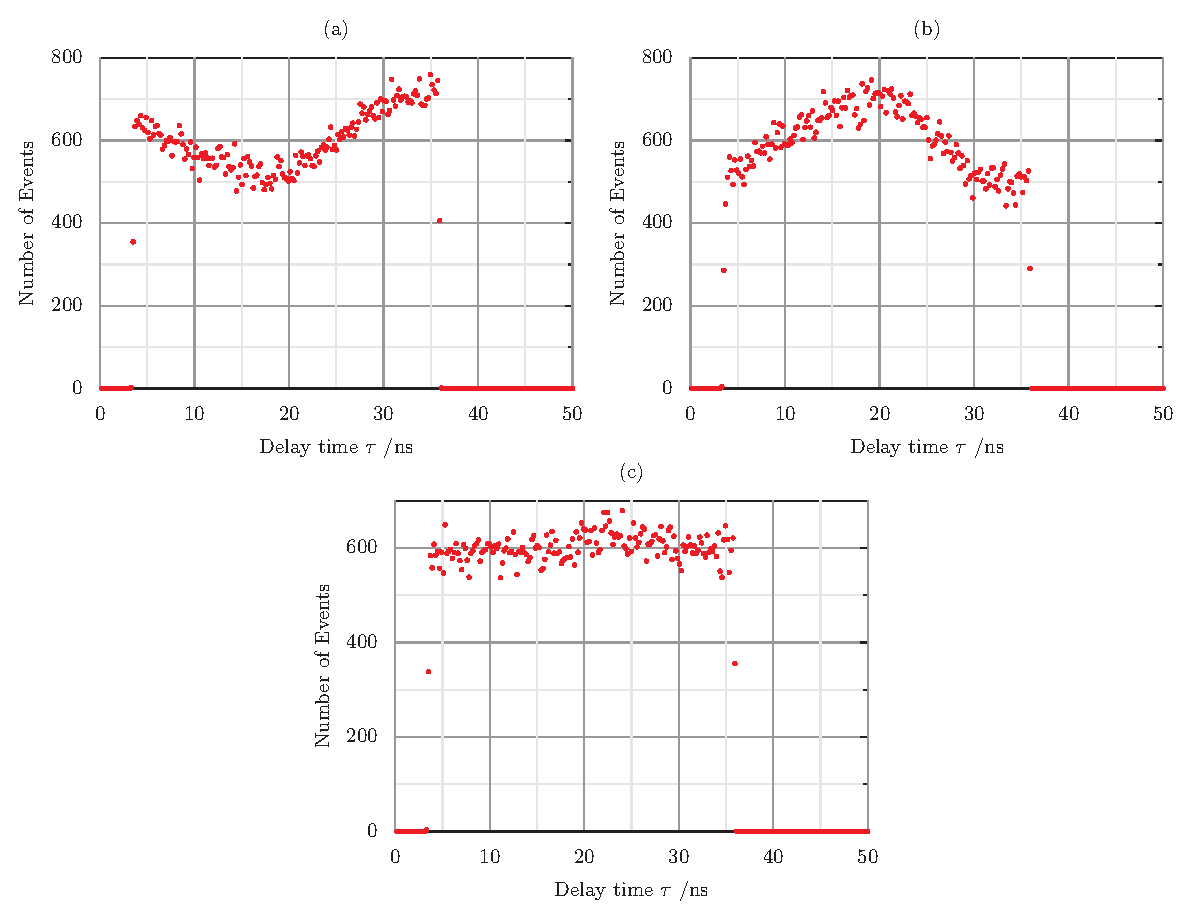
\includegraphics[width=14.5cm]{chapter6/rfcorr/rfexplots}
\caption[RF-photon compensation signals]{Recorded RF-photon compensation signals for different field compensations. The number of recorded photons is shown as a function of time since the beginning of an RF-cycle (delay time). In the case of good field compensation, the photon arrival times are independent of the RF cycle. (a) under-compensated, (b) over-compensated, (c) well compensated. The origin of the cut-off values are discussed in the text. Plot from A. Myerson's first year report \cite{Myerson2007}.}
\label{rfcorrelation}
\end{figure} 

To compensate in the X direction (across the trap) a secondary, ``vertical'' 397\nm\, beam was used, with a component of its wave vector in the X direction. Thus, after compensating in the Z and Y directions with the horizontal beam, the vertical beam is turned on and the RF-photon correlation is used to check the X-compensation. The compensation is adjusted by putting a voltage difference between the lower and higher set of DC electrodes. This voltage difference was usually of the order of 0.9\V. 

With the RF-correlation method, the Z-Y compensation can be set to within $\pm 0.02\V$ of the optimal value. In the X direction, the compensation can achieve within $\pm 0.05\V$ of the optimal value. Using the numerical model of the trap, these values correspond to electric field components $\pm 5\V/\m$ in the Y direction and $\pm 20\V/\m$ in the X direction, respectively. The lower sensitivity to micro-motion in the X direction is due to the higher background scatter level of the vertical 397\nm\, beam. 

The field compensation generally changes over time, depending on the environment and the experiments conducted. While improving the field compensation, a number of factors affecting it were identified. 

Figure~\ref{fig:lablightingcompensate} shows the effect of ambient light in the laboratory on the field compensation. Turning on the lighting in the laboratory changes the field compensation in an immediate and reversible manner. 

A possible source of this effect is the exposed silicon on the face of the chip surface. The doped high resistivity silicon (below a thin $\mbox{SiO}_x\mbox{N}_y$ layer) is inherently sensitive to light in the visible range. In practice, it might act as an imperfect photodetector on the chip, where the created electron-hole pairs are not collected, just separated. These electrons and holes can, however, distort the field in the trapping region because of their proximity. 

This theory, however, was not tested at the time, as the issue is easily circumvented by turning off the lights during the experiments. The next generation of the Sandia trap design features a gold-plated front face. Comparing the behaviour of the two designs will help our understanding of the effect of the exposed silicon surface on the trap operation.


\begin{figure}[h!t]
\centering
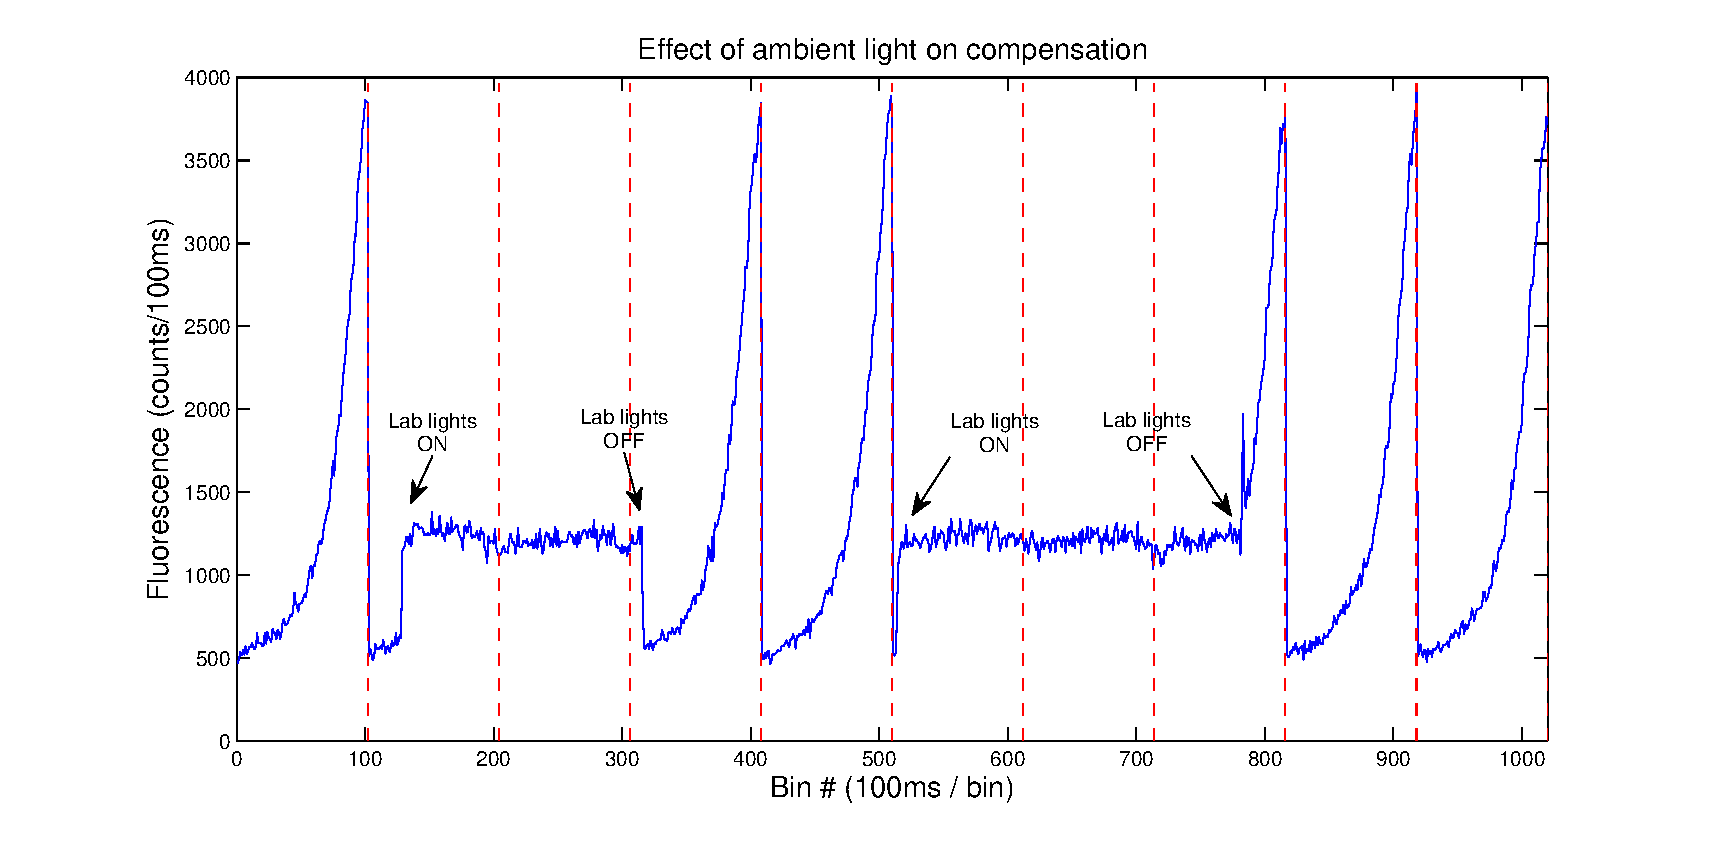
\includegraphics[width=14.5cm]{chapter6/lablights/lablights3}
\caption[Effect of ambient light on ion compensation]{Recorded fluorescence signal during repeated scans of the 397nm laser from red detuned to close to resonance with a range of approximately 132\MHz. The ion motion is compensated beforehand. The dashed vertical lines separate the scans. The laboratory ambient lighting was turned on and off during the sequence, as shown on the plot. The signal during those periods has a highly Doppler-broadened profile, and is effectively flat in the scanned frequency region. }
\label{fig:lablightingcompensate}
\end{figure} 


Figure~\ref{fig:loadcompensation} shows the effect of repeated ion loading on the field compensation. After successive ion loads, larger and larger compensation fields were required. On the other hand, long-term ion storage did not change the compensation significantly. The observed behaviour can be explained by charge build-up during the ion loading. This could be due to the photoionisation lasers (especially the 389\nm\, beam, having the shortest wavelength), or the \CaI{} oven. However, repeated tests failed to show any effects of the laser beams, even when directed onto the electrodes for extended periods. The operation of the \CaI{} oven, on the other hand, noticeably changes the field compensation, even after after a few (3-5) minutes of operation. 

The exact nature of the oven's effect has not been identified. One theory was charge building up on the trap due to thermal electron emission of the \CaI{} oven. To eliminate this effect, the oven was biased with a large positive voltage (larger than any voltages on the DC electrodes, of the order of 30\V) with respect to the common ground of the rest of the system. The positive voltage should act as a sink for the thermal electrons, reducing the charge build up, and thus the change in field compensation. This method, however, failed to achieve any observable reduction of stray electric fields, and was abandoned after a trial period of a few weeks.


\begin{figure}[h!t]
\centering
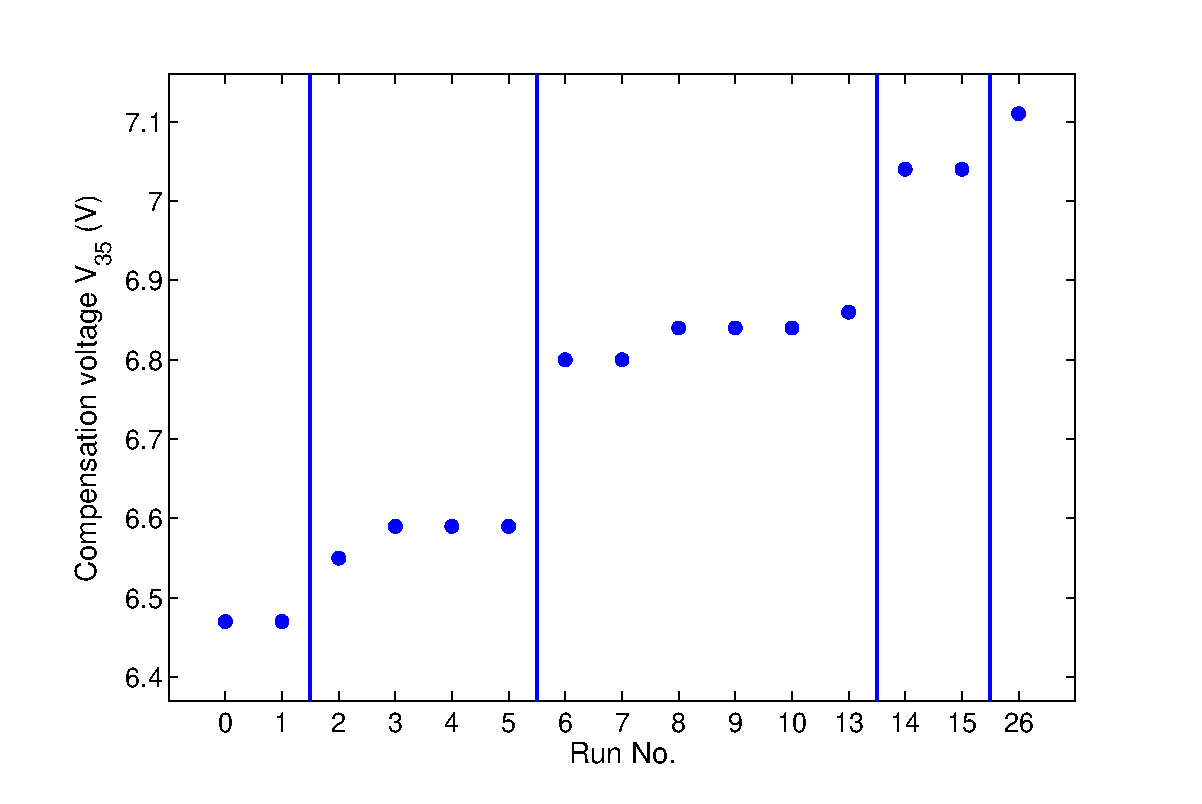
\includegraphics[width=12.5cm]{chapter6/loadcompensation/loadcompensation}
\caption[Changing compensation when reloading]{Figure showing the changing compensation when reloading. The voltage on the electrode pair \#3 and \#5 is plotted as a function experiment number. The compensation is checked before every experiment and adjusted if necessary. The vertical lines represent lost ion and reloaded trap. Thus, all experiments between two vertical lines are done with the same ion. The approximate time scale is 3-4 minutes for a compensation check and experimental run, 4-5 minute for loading an ion. It is clear that large changes happen in the compensation when reloading. }
\label{fig:loadcompensation}
\end{figure} 



\section{Lifetime}

In the initial experiments the ion lifetime in the trap was very short, only of the order of tens of seconds even with the cooling lasers on. This was long enough to observe the ions and do basic micro-motion compensation, but unsatisfactory for any more complex experiments. To improve the situation, experiments were conducted to check the effect of different ion loading methods on the ion lifetime.

As qualitative tests failed show any change in the micro-motion compensation caused by the applied laser beams, the lasers were not considered to be the immediate cause of the short lifetime. The \CaI{} oven, however, had a significant effect on the field compensation (as  was shown in the previous section), and it could be a more significant factor in causing instabilities in the trap, leading to the loss of trapped ions.


The results of the experiment are analyzed in terms of an estimated survival function. The survival function is the probability of the ion staying in the trap longer than $t$:
\be
S(t) = P(\tau \geq t)
\ee
where the ion lifetime is $\tau$.

The survival function was estimated using the non-parametric Kaplan-Meier (or product limit) estimator \cite{Kalbfleisch2002}:
\be
\hat S(t) = \prod_{t_i < t} \frac{n_i - d_i}{n_i}
\ee
where $t_i$ is the $i$th recorded distinct ion lifetime, $n_i$ is the number of ions with lifetime longer than $t_i$, and $d_i$ is the number of ions with lifetime equal to $t_i$. The variance of the Kaplan-Meier estimate of the survival function is calculated as \be
\mbox{Var}(\hat S(t)) = \hat S(t)^2 \sum_{t_i<t} \frac{d_i}{n_i(n_i-d_i)}
\ee
which is used to calculate the confidence interval of the estimated half-probability lifetime (the time up to which half the ions survive).


Two sets of tests were conducted, changing different aspects of the ion loading procedure. In the first experiment, the effect of different oven drive currents were tested. Three different currents (5.25\A, 5.5\A, 5.75\A) were used. During the experiment, one of the currents was set, and, when the oven temperature stabilised, ion loading was attempted. Temperature stability was assumed when the electric resistance of the \CaI{} oven stopped changing. Once an ion had been loaded into the trap, the photoionisation beams were blocked, and the fluorescence signal was recorded until the ion was lost. The observation was repeated with a large number of ions. After a certain time (10-15 minutes) a different oven current was set, and the observations repeated. The oven current was changed a large number of times, and the complete data set for each of the oven currents comes from multiple observation sequences. The field compensation was checked at the beginning of the experiment, and was not changed during the observations. The measured ion lifetimes were extracted from the recorded fluorescence signal.


The results of the first experiment are plotted in Figure~\ref{fig:lifetimeplot_temperature} and listed in Table~\ref{tab:lifetimes} (series \#1-3). The ions had a longer lifetime in the trap when the \CaI{} oven was operated at a lower temperature (lower drive current). The half-probability lifetime was in the order of 300\s\, for the low current loading (5.25\A), while it was $<$100\s\, for the higher current (5.5\A, 5.75\A) cases. Thus, a lower \CaI{} oven current at the loading improves the ion lifetime. 

During these experiments, the photoionisation beams were blocked once an ion was loaded, to stop excess ion creation in the trapping area, but the \CaI{} oven was on during the whole experiment, emitting neutral \CaI{} atoms.

We now turn to our second experiment, in which we compared two different ion loading methods. The first method maintained the operating oven temperature after an ion had been trapped (as in the previous experiment). In the second method after an ion was trapped, the \CaI{} oven drive current was lowered from 5.25\A\, to 2\A\, to stop the emission of \CaI{} vapour. The 2\A\, current was considered low enough to stop \CaI{} emission, while maintaining an oven temperature that can be raised quickly to the operating temperature.

During the experimental sequence 10-15 minutes long sessions of the two different ion loading methods were alternated. The recorded lifetimes of a given loading method are then combined into a single data set. 

In the sessions when the oven is turned down after loading, there was a delay of about 1-2 minutes before loading an ion, because the oven had to heat up. This results in a smaller number of observations (28 ion lifetimes) compared to the ``always-on'' setting (48 ion lifetimes). 

Figure~\ref{fig:lifetimeplot_ovens} shows and Table~\ref{tab:lifetimes} (series \#4-5) lists the result for the experiment of turning down/leaving on the \CaI{} oven after trapping an ion.  The survival probability is slightly higher in the case when the oven is turned down, though the difference in the lifetimes is smaller than that caused by higher oven currents.

\begin{table}[t]
\begin{center}
\begin{tabular}{|l|c|c|}
\hline \textbf{Experimental series}  & \textbf{No. of ions} & \textbf{Half-probability lifetime (s)} \\ 
%\hline  \#1: $I_{\mbox{oven}}$ =  5.25\A &  361 \\ 
%\hline  \#2: $I_{\mbox{oven}}$ = 5.5\A  &  73  \\ 
%\hline  \#3: $I_{\mbox{oven}}$ = 5.75\A &  29  \\ 
%\hline  \#4: $I_{\mbox{oven}}$ = 5.25\A &  286 \\ 
%\hline  \#5: $I_{\mbox{oven}}$ = 5.25\A\, - turned down after loading &  579 \\ 
\hline  \#1: $I_{\mbox{oven}}$ =  5.25\A & 40 & 362 [225...466] \\ 
\hline  \#2: $I_{\mbox{oven}}$ = 5.5\A  & 53 & 74 [49...92] \\ 
\hline  \#3: $I_{\mbox{oven}}$ = 5.75\A & 72 & 29 [23...56] \\ 
\hline  \#4: $I_{\mbox{oven}}$ = 5.25\A & 48 & 289 [190...453] \\ 
\hline  \#5: $I_{\mbox{oven}}$ = 5.25\A\, - turned down & 28  &  581 [399...905] \\ 
\hline 
\end{tabular} 
\caption{Experimental lifetimes of ions, for different \CaI{} oven currents. The numbers in the square brackets show the 95\% confidence interval of the ion lifetime. The different experiments are described in the text.}
\label{tab:lifetimes}
\end{center}
\end{table}

After these experiments we observed even longer average ion lifetimes in the trap than shown in the results above. This can partly be attributed to gaining more experience in operating the trap and performing the field compensation. After a few weeks of operating the trap, we regularly observed ion lifetimes of tens of minutes. The longest observed lifetime is over 2 hours, even while performing different experiments, e.g. probing trap frequencies as described in the following section.

A tentative explanation of all these results is as follows. The lifetimes of order 1 minute observed at oven current 5.5\A\, is consistent with loss by collisions with atoms and molecules in the background gas, according to the following argument. The studies in Chapter~\ref{chapter:firstobs} permit us to estimate the oven temperature T = 625\K\, when the current is 5.5\A\, (see Figure~\ref{fig:temp_current}). Equations~\ref{eq:n_n0}, \ref{eq:np} and \ref{eq:pt}  give the number density of Ca atoms in the atomic beam near the trap region as
\[
n_{\rm beam} = 1.9 \times 10^{11} \, \m^{-3}
\]

Meanwhile figure 5.12 shows the pressure at the ion gauge was then approximately  $5 \times 10^{-10}$\torr. Other studies suggested the ratio between pressure at the trap and pressure at the ion gauge is about 3, so the pressure at the trap could be of order $10^{-9}$\torr\, (the ion gauge is imprecise at measuring \CaI{} pressure). Assuming this gas is at room temperature, it has a number density
\[ 
n_{\rm gas} = \frac{p}{k_B T} \simeq 3.3 \times 10^{13} \, {\rm m}^{-3}
\]
The fluorescence scans would show a Gaussian profile if the Ca at the trap were predominantly in the form of a Maxwellian gas rather than a beam, which suggests the background gas is not predominantly \CaI{}, but whatever it is, it can lead to collisional loss. 

Collisions between \Ca{} ions and neutral \CaI{} atoms involve various effects, including charge exchange and glancing elastic collisions via the comparatively long-range induced-dipole potential. Preliminary calculations \cite{Steane2008} show, for example, that for the $1/r^4$ \CaI{}--\Ca{} interaction potential the Langevin distance is $b_L = 1.6$\nm\, and 1.3\nm\, for incident atoms at 293\K\, and 625\K\, respectively. Collisions at an impact parameter below $b_L$ can be expected to eject an ion from the trap. Thus the collisional loss cross section is about 100 times larger than would be implied by a simple hard-sphere model. Values around 1\nm\, are obtained for N$_2$ molecules and H$_2$O molecules. Using this number, the loss rate is estimated as $\pi b_L^2 n \bar{v} = 0.04$, i.e. one per 26 seconds. This is of the order of the observed value.

In later work the background pressure in the trap was substantially lower, and this could be the explanation for the substantially longer lifetimes observed.



\begin{figure}[h!t]
\centering
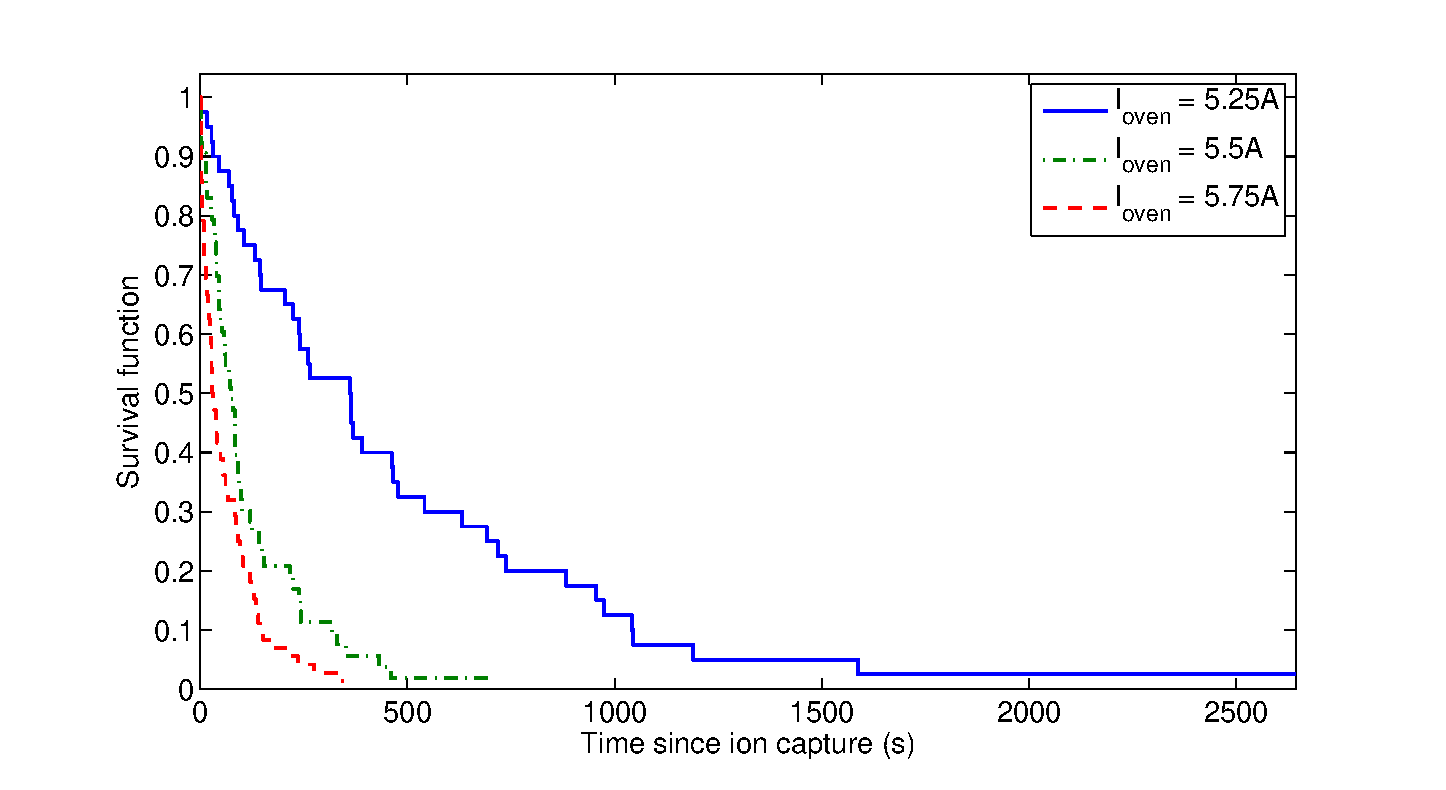
\includegraphics[width=14.5cm]{chapter6/lifetime/lifetime_temps}
\caption[Effect of \CaI{} oven temperature on ion lifetime]{The experimental survival function of the ions in the trap, for different oven temperatures while loading. The photoionisation beams were blocked after ion capture, the fluorescence was observed until the ion was lost.  High oven drive current (high oven temperature) shortens the ion lifetime. \cversion}
\label{fig:lifetimeplot_temperature}
\end{figure} 

\begin{figure}[h!t]
\centering
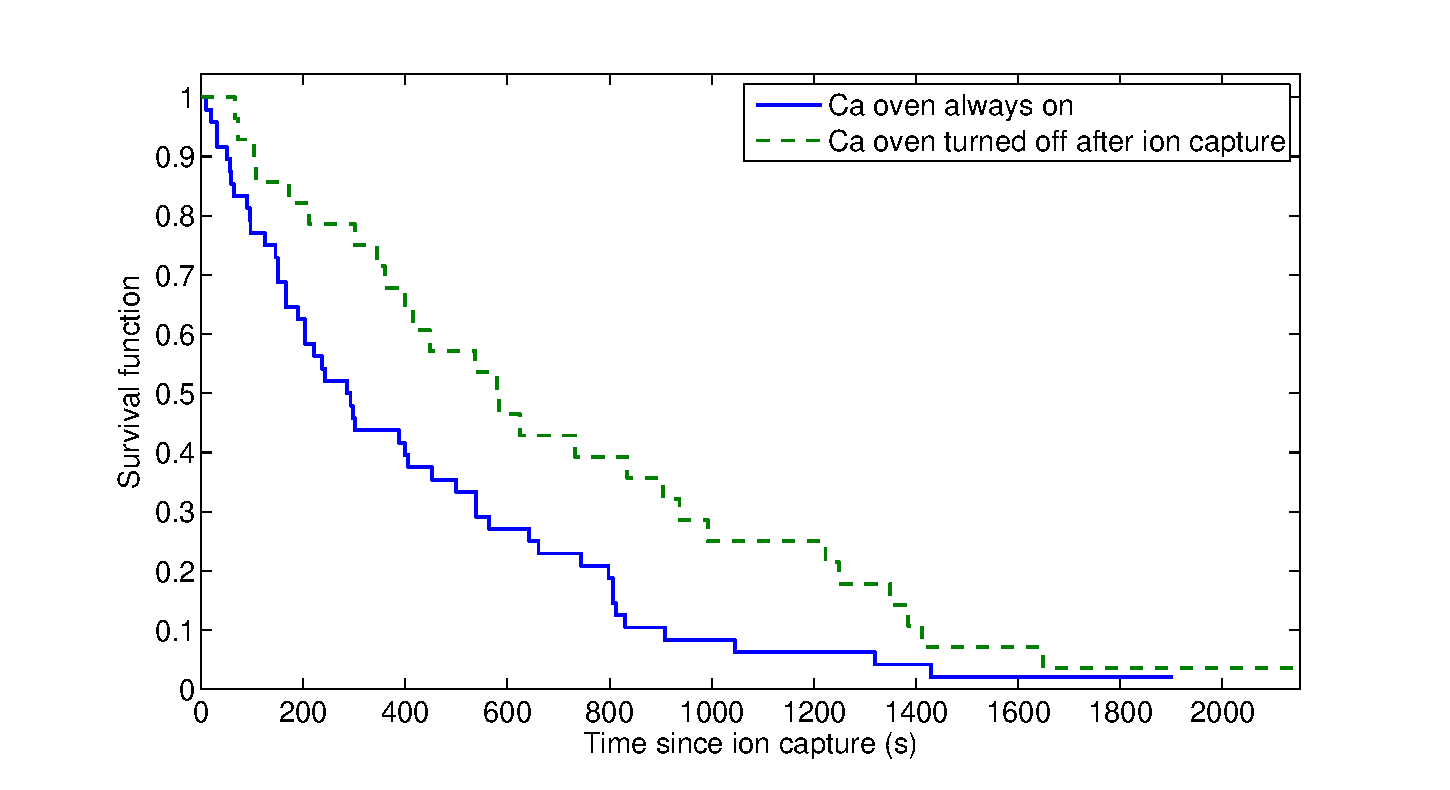
\includegraphics[width=14.5cm]{chapter6/lifetime/lifetime_oven}
\caption[Effect of turning off \CaI{} oven on ion lifetime]{The effect of reducing \CaI{} oven drive current after ion capture on the ion lifetime. The survival function is plotted for the two different loading methods. The \CaI{} oven generally cools down in a matter of seconds, and stops emitting \CaI{} vapour, as was verified by pressure measurements. \cversion}
\label{fig:lifetimeplot_ovens}
\end{figure} 



\section{Vibrational frequency measurements}
\label{sec:ticleexperiment}

The axial and radial trap frequencies are important parameters, crucial for many experiments with single and multiple ions. Computer simulation of the fields in the ion trap can provide estimates, but our models of the trap have to be validated, by comparing predictions to experimentally observed frequencies.

One uncertainty in the computer models is the trap geometry, since the actual manufacturing process might have deviated from the initial plans. Also, there can be conducting materials in the assembled setup, not accounted for in the plans, and their position is not known with good accuracy. Examples of these are gold-plated surfaces on the back side of the Sandia trap, or the out-of-plane compensation electrode added to the system during the system assembly.
%add sectionto reference???


Another uncertainty is the exact value of the applied RF voltage. The RF voltage depends on the Q-value of the helical resonator, which cannot be accurately measured outside the vacuum can. By experimentally determining the radial trap frequencies, the comparison with computer models yields the effective voltage on the RF electrodes. Then the Q-value can be determined since the applied input voltage of the helical resonator is known. 

To probe the trap frequencies, an AC ``tickle'' voltage oscillating at a frequency close to the expected ion vibrational frequencies was applied to some of the DC electrodes. The frequency was scanned, and the fluorescence signal was recorded. When the tickle frequency was in resonance with any of the trap frequencies, the ion's motion was excited and the fluorescence signal changed. 

When the 397\nm\, laser is tuned close to the atomic transition (for example, to the half-fluorescence point on the red side of the transition), an increase in the ion's motion will cause a dip in the fluorescence. This dip, however, is quite small compared to the original fluorescence level, because there has to be very large Doppler-broadening of the profile to have a significant drop in fluorescence at such small detuning. Better results are achieved when the 397\nm\, laser is detuned further from the atomic fluorescence. When stray fields are properly compensated and the laser is tuned to -200\MHz\, (red detuning), the observed fluorescence is almost at the background scatter level (see Figure~\ref{fig:397compensationscans}). At such detuning, an increase due to the Doppler-broadening of the spectra will result in a large increase of the fluorescence. Figure~\ref{fig:ticklescan} shows an example of such a tickle scan, when exciting the ion's radial frequencies.

First the axial trap frequencies were probed. The RF voltage is applied to the electrode pair \#2, grounded in most of the other experiments. A Tenma Jupiter 2010 2\MHz\, function generator was used to provide 8\Vpp\, on its 50\Ohm\, output, to excite the ion's axial motion. The frequency of the function generator was controlled by the experimental control computer via the function generator's DC input. The frequency was scanned linearly, with good repeatability.

Results of the scans, showing the axial trap frequency as a function of applied DC electrode voltages, are plotted in Figure~\ref{fig:axialtickle}. Trap frequency predictions from computer simulations are also shown. The predicted frequencies have a similar DC electrode voltage dependence to the experimental values, but they are about 10\% lower. This discrepancy is probably due to the imperfection of the computer model of the trap, as discussed in Section~\ref{sec:sandiaintro}.


%The first is the uncertainty of the exact geometry and placement of the electrodes and the gold-plated back plane. To properly evaluate the effect of adjustments of the geometry would require additional simulations, and these would be impractical anyway because of the large number of parameters. The second issue is the limitation of the software used. It is capable of calculating electrode structures up to 6000 elementary segments. Tests with different total segment numbers suggested that this is barely sufficient to ensure converging results for such a complicated structure as the Sandia trap. In the future, a different software package is likely to be employed, but this was not available for us at the time of the experiments. Nevertheless, for most purposes the current model is adequate, and for any experiment requiring high precision trap frequency values, the tickle can be performed beforehand.



To measure the radial trap frequencies a new signal generator was needed, as the frequencies were expected to be higher than the 2\MHz\, limit of the Tenma Jupiter 2010. An Agilent 33220A 20\MHz\, arbitrary waveform generator (AWG) was used, and the output of the function generator was connected to the extra compensation electrode (see hardware description in Section~\ref{subsec:sandiatrap}). The applied RF voltage was a sine wave function, with 250\mV peak-to-peak. The frequency scan was pre-programmed in the AWG, and the scanning was triggered by the experimental computer. Then the timing (bin number) of the recorded fluorescence contains the relevant frequency information. 

When using the ``horizontal'' 397\nm\, laser beam, the motion is observed only in the Y direction; while using both the ``horizontal'' and the ``vertical'' beams, both peaks corresponding to the X and the Y radial frequencies are present in the scans. Scans using only the ``horizontal'' beam have better signal-to-noise ratio due to the smaller amount of background scatter. Thus the first scans to roughly locate the radial frequencies were done using the ``horizontal'' beam only. Once the correct region had been found, both beams were turned on to measure the two radial frequencies in a single run.

Figure~\ref{fig:radialtickle} shows the combined results of the tickle scans of the radial frequencies, as a function of the RF drive voltage. The best fitting simulation results are also plotted. The fitting is done adjusting a single parameter, the Q-value of the helical resonator, to get the amplitude of the RF voltage on the RF rails from the drive voltage. The fit gives Q-value of 21, which is very close to the expected Q-value of 20 (by measuring the voltage just outside the vacuum chamber after the resonator).

The radial frequency in the X direction can be fitted much better than that in the Y direction. The discrepancy between the measured and simulated values is probably due to the incomplete knowledge of the shape of slot's sides, whose gold coating provides a large grounded DC electrode. Nevertheless, as in the case of the axial trap frequency, the predicted and measured frequencies are largely consistent. 
%%% there was a \begin{center} here, why?


\begin{figure}[h!t]
\centering
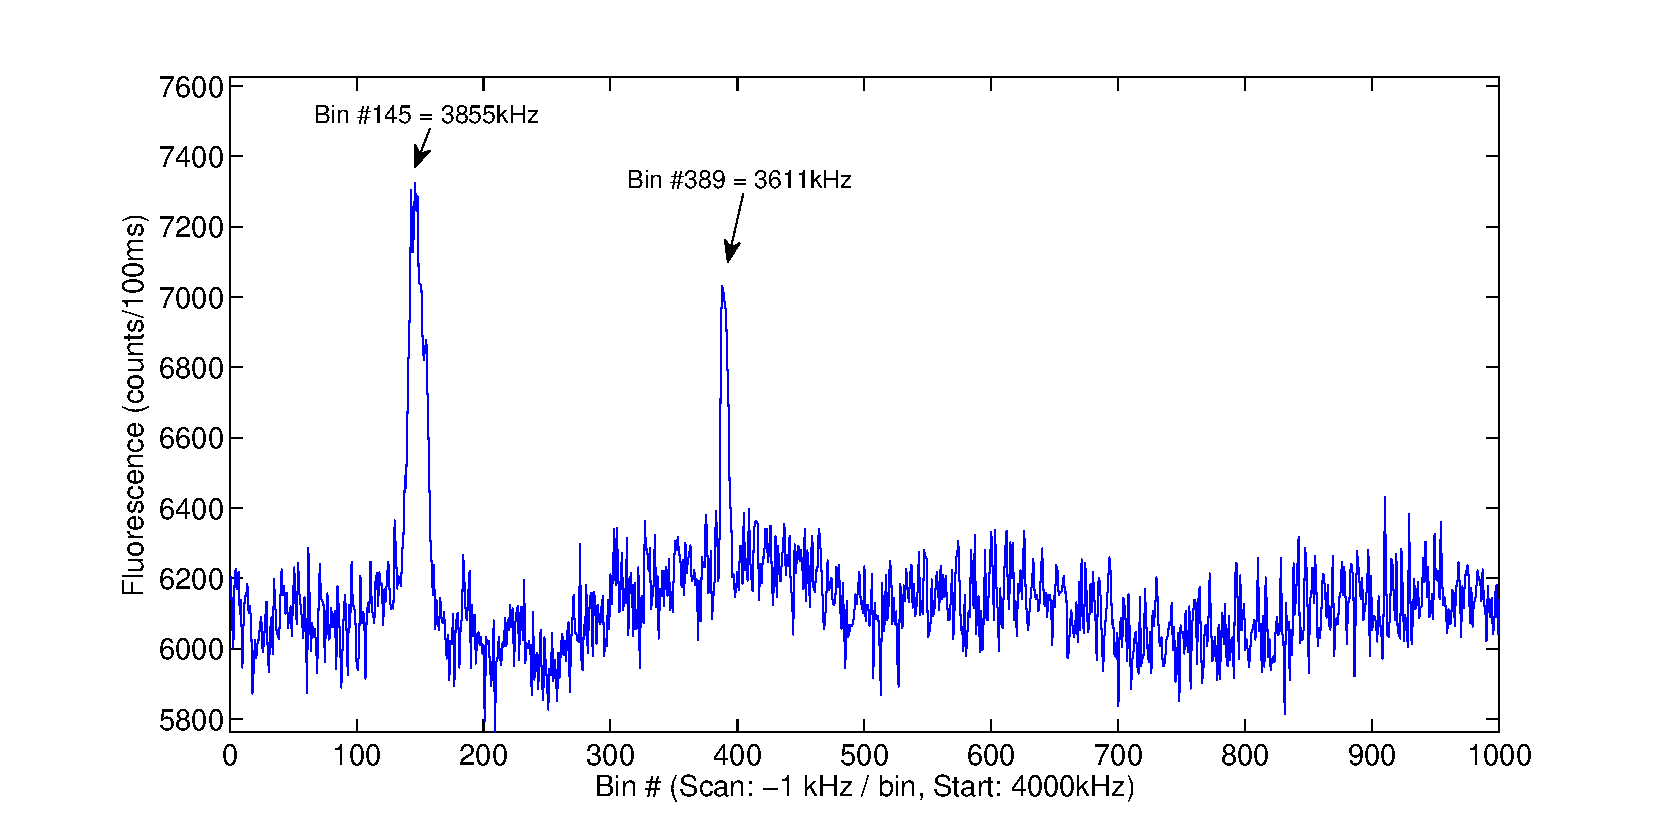
\includegraphics[width=13.5cm]{chapter6/tickle/ticklescan}
\caption[Example scan of tickle experiment determining trap frequencies.]{Example of scan in the tickle experiment to determine the radial trapping frequencies. The fluorescence is recorded as a function of the tickle frequency. The experiment was done having both ``horizontal'' and ``vertical'' 397\nm\, beams on. When the ``vertical'' beam was turned off, only a single peak was observed (at the higher frequency of the two), determining which peak corresponds to the X and Y direction, since the ``horizontal'' beam alone is only sensitive to the ion's motion in the Y radial direction. The peak's position is determined with precision ~$\pm 15 \kHz$.  ($V_{RF} = 8$Vpp)}
\label{fig:ticklescan}
\end{figure} 



\begin{figure}[h!t]
\centering
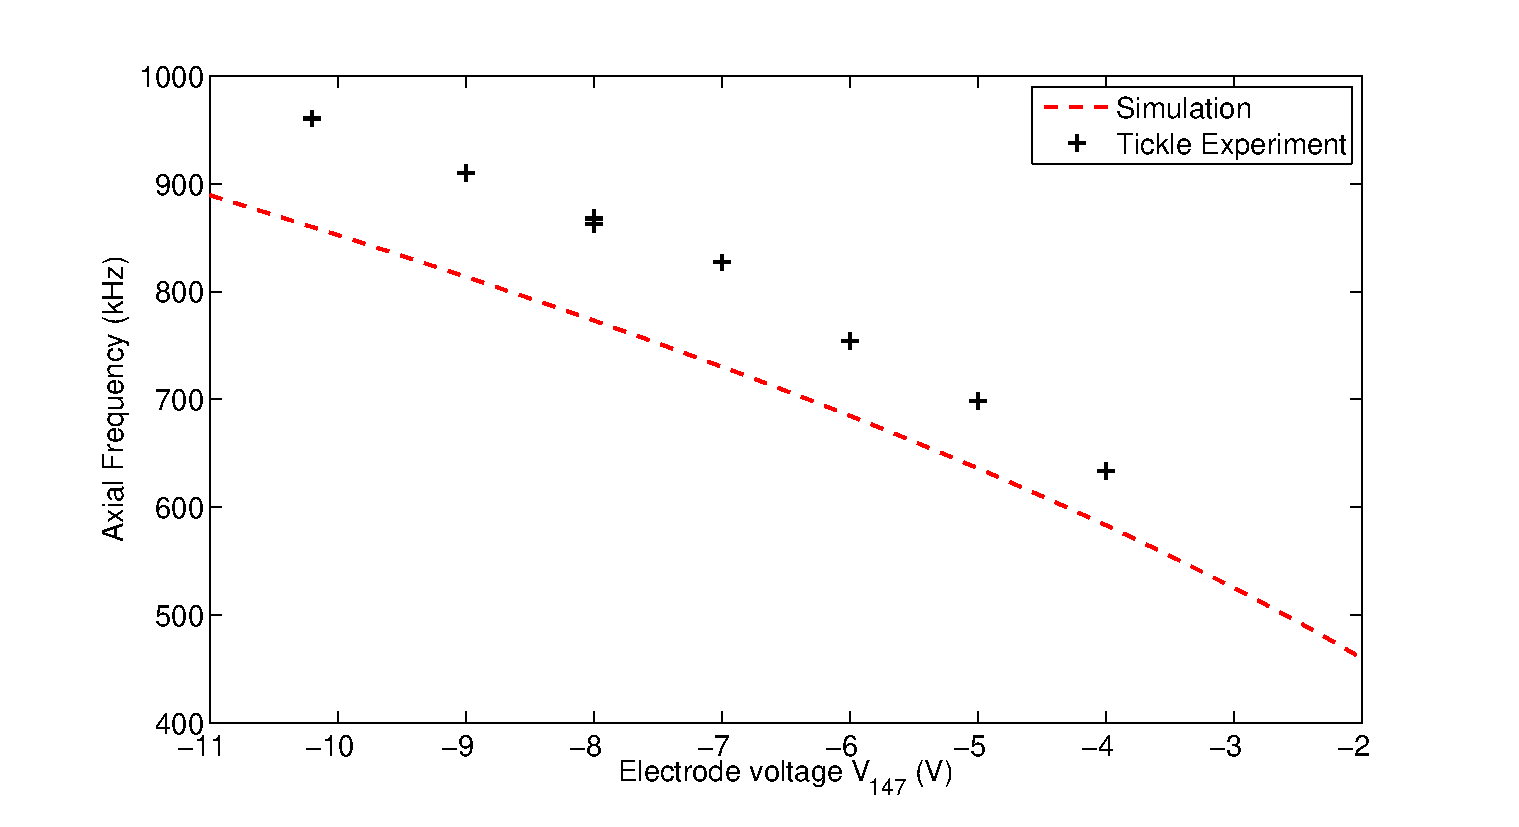
\includegraphics[width=13.5cm]{chapter6/tickle/axialtickle}
\caption[Axial trap frequency]{Measured axial frequency as a function of voltage on DC electrode pairs \#1,\#4 and \#7, while the other DC electrode voltages and the RF amplitude were kept constant. The measured frequencies are compared to simulation results. The simulation reproduces the correct shape of voltage dependence, but not the correct values. The discrepancy is probably mostly due to uncertainty in the exact geometry, particularly the placement of the electrodes and the gold-plated back plane.}
\label{fig:axialtickle}
\end{figure} 

\begin{figure}[h!t]
\centering
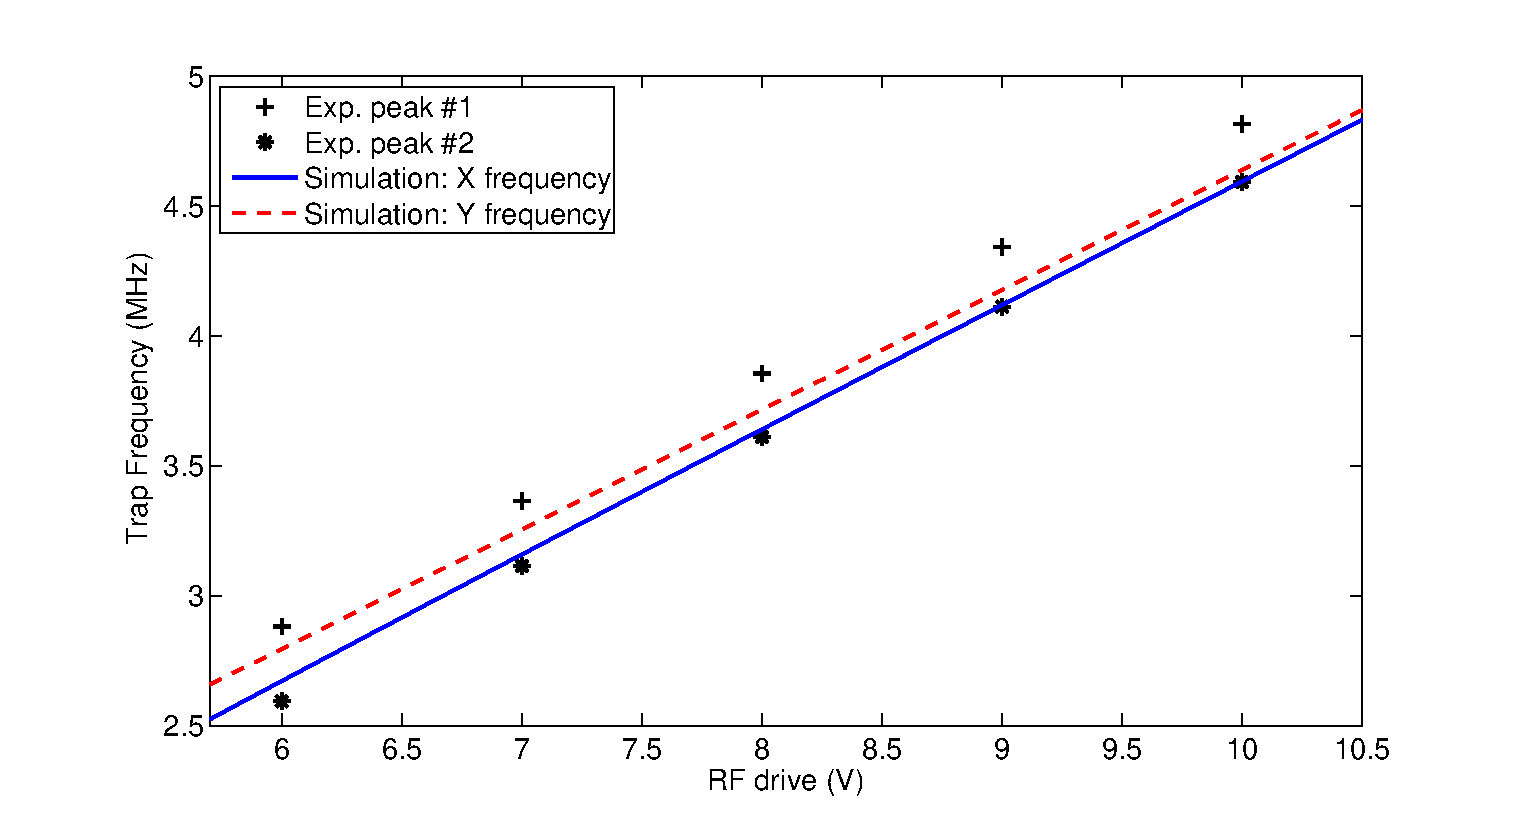
\includegraphics[width=13.5cm]{chapter6/tickle/radialtickle_drive}
\caption[Radial trap frequencies]{Measured radial trap frequencies as a function of RF drive voltages, compared to simulated values. The simulated trap frequencies are fitted to the measurements to infer the Q-value of the helical resonator (the conversion factor between the RF drive voltage and the peak-to-peak RF amplitude on the electrodes). According to the fit, the Q-value is 21, which is close to the expected value of 20. The discrepancy between the fitted and measured trap frequencies is probably mostly due to uncertainty in the exact geometry of the trap.}
\label{fig:radialtickle}
\end{figure} 



\section{Loading multiple ions}
\label{sec:multiions}

In practice one wants to be able to store multiple ions in the same trapping region, so that they can interact with each other. In most quantum computing schemes it is sufficient to store a pair of ions in a single trapping region, as all quantum algorithms can be implemented using single-qubit and two-qubit quantum gates. 

We experimented with multiple ion loading in the Sandia trap with partial success. During normal single ion loading as described earlier in this chapter, when the 854\nm\, deshelving beam was used, multiple ions were loaded into the trap occasionally, but their occurrence was unpredictable and had a very short lifetime. A recorded fluorescence signal of such multiple loading is shown in Figure~\ref{fig:multiload}.

In controlled multiple ion loading experiments some changes were made to the trapping fields that were believed to improve the loading success rate and/or multiple ion lifetime. The RF supply voltage was lowered from the usual 8\Vpp\, ($\sim 84$\V\, amplitude on the RF electrodes) to 6\Vpp\, ($\sim 63$\V\, amplitude on the RF electrodes) or lower. This corresponds to radial trapping frequencies of 3\MHz\, or lower. The DC voltages were also changed to provide a lower axial trapping frequency (from the usual 800-900\kHz\, to 300-500\kHz). The lowest trap frequencies were used when we attempted to optically resolve the multiple ions. The measurement of the ions' separation as a function of the electrode voltages can further validate the simulation model of the trap.

Using lower trap frequencies, pairs of ions were loaded repeatedly, with reasonable reproducibility. The loading rate was of the order of a pair every 3-4 minutes. However, the pair lifetime was very short. While by this time in our experiments single ions were kept for more than 2 hours, the longest observed pair lifetime was $\sim$2 minutes. 

This short lifetime was sufficient, however, to take a series of pictures of the ions with a CCD camera and calculate their separation, see Figure~\ref{fig:pairions}. The results are in reasonable agreement with the expected values from the simulation of the trap. 





%%%%%%%%%%%%%%%% Praise
%
%Loading, cooling and compensation in microfrabricated ion traps is much harder than in the tried and tested macroscopic designs. This difficulty is illustrated by the fact that of the four ion trapping groups using the Sandia design, only our group and the NIST ion trapping group were able to trap ions and carry out experiments on them. Our efforts provided useful data on the pilot design of the Sandia trap and allowed measurements of heating rates and experiments of ion shuttling (see next chapter).
%


\pagebreak

\begin{figure}[t]
\centering
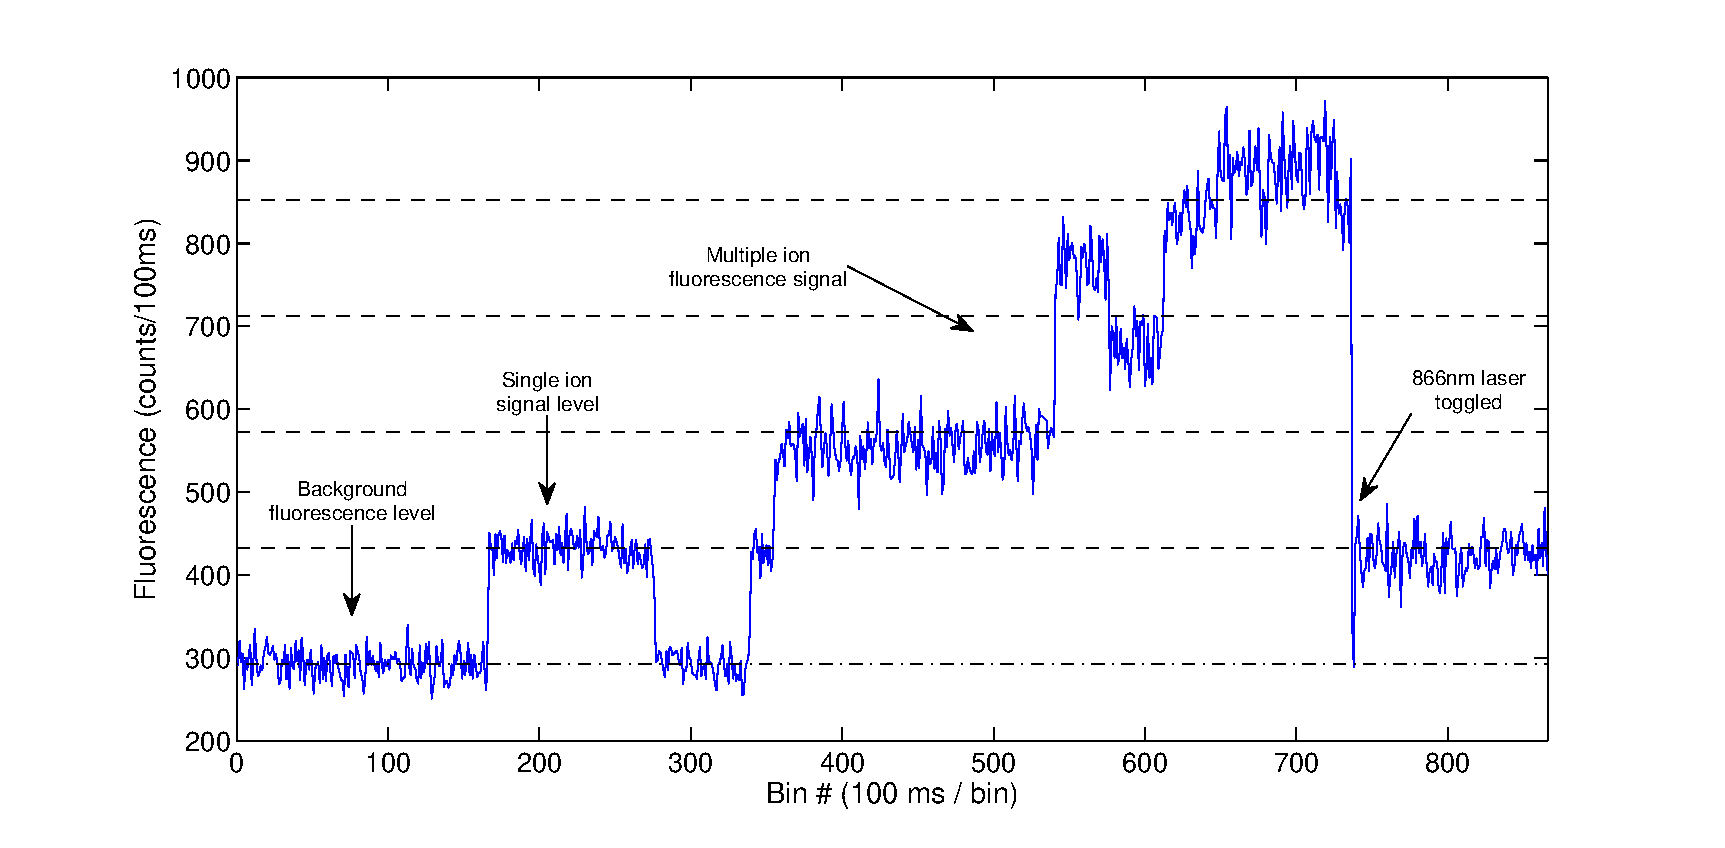
\includegraphics[width=14.5cm]{chapter6/multiload/multiload3}
\caption[Fluorescence signal of multiple loaded ions]{Fluorescence signal during ion loading. First a single ion is loaded. The \CaI{} oven, photoionisation lasers and 854nm re-pumping laser were left on.  The signal shows a quantum jump-like  behaviour, suggesting that multiple ions were trapped. Then the 866nm laser was toggled on/off quickly, which turns off the Doppler cooling of the ions for a short period of time. On the plot the \textit{dash-dotted} line represents the approximate background count level, while the \textit{dashed} lines show the approximate 1,2,3,4 ion signal levels, based on the single ion signal.}
\label{fig:multiload}
\end{figure} 


\begin{figure}[!ht]
\centering
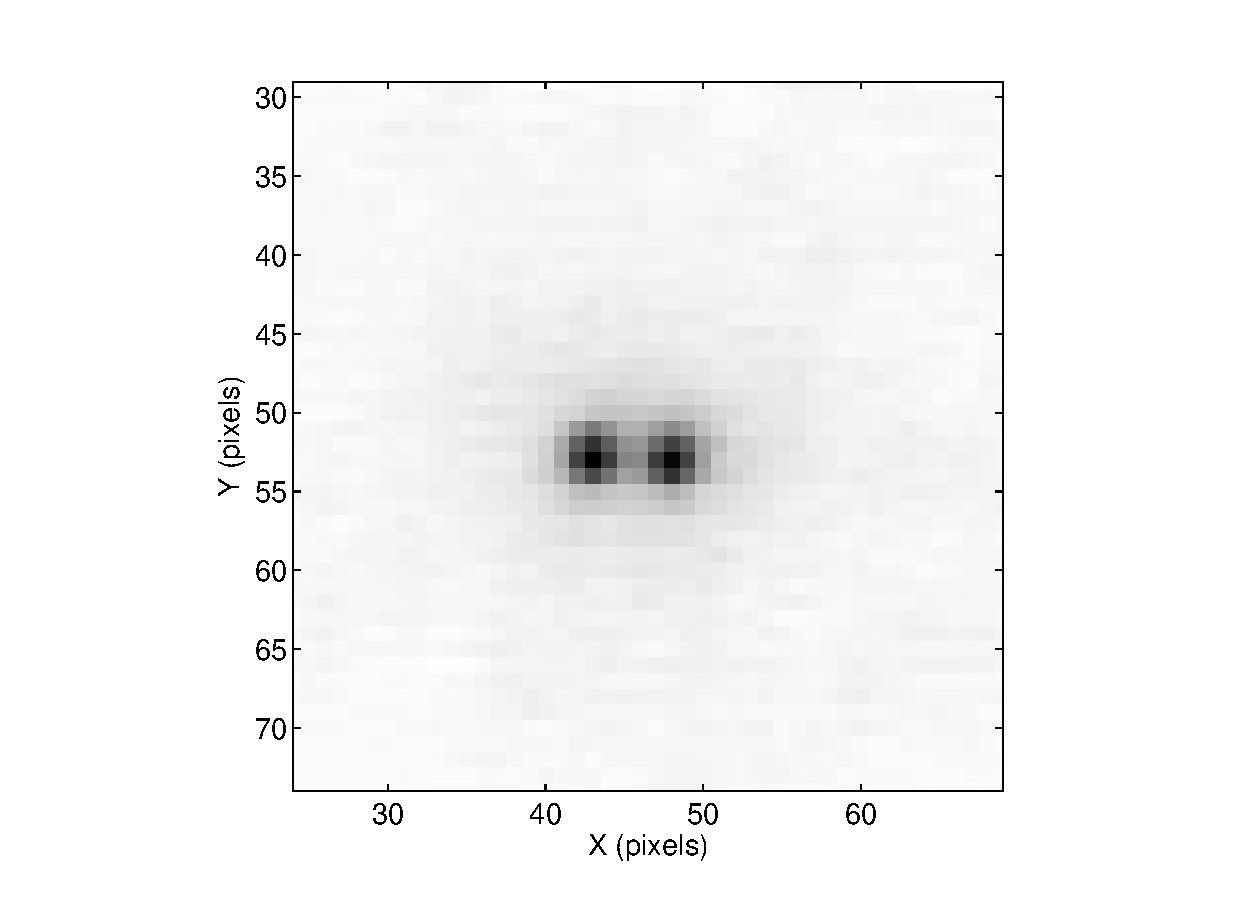
\includegraphics[width=11cm]{chapter6/twinion/twinionpic}
\caption[Picture of a pair of ions in the trap]{Picture of a pair of ions in the trap. Averaged over 12 pictures, taken with the EEV intensified CCD camera. Axial trap frequency $\sim 317\kHz$, Radial frequency $\sim 2.7\MHz$ ($V_{RF} = 6\V$ peak-to-peak), length-scale of pictures: 15.3\um / pixel. With the imaging system's 8x magnification taken into account, the ions have a separation of $\sim 9.6 \um$.}
\label{fig:pairions}
\end{figure} 


%%%%%%%%%%%%%%%%%%%%%%%%
% Dummy Picture template

% \begin{figure}[h!t]
% \centering
% 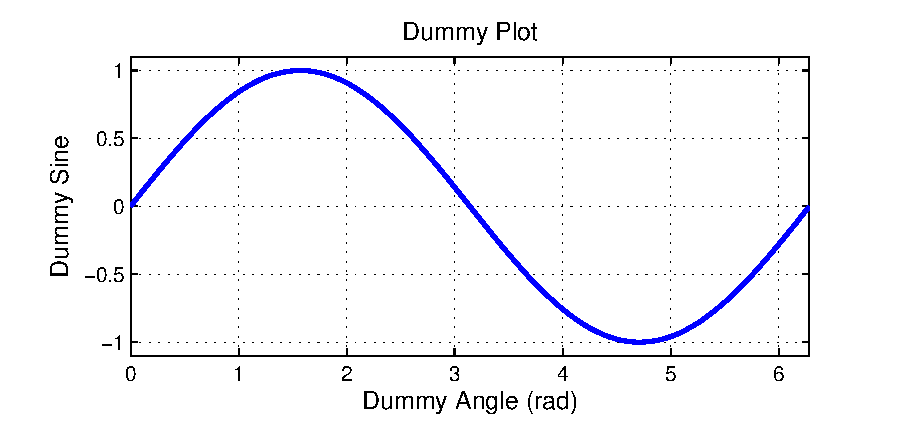
\includegraphics[width=8cm]{dummy}
% \caption[]{}
% \label{dummy}
% \end{figure} 
